\chapter{Metodologia}


A metodologia está dividida nas seguintes etapas:

\subsection{Coleta de dados}

A busca por dados brutos das duas classes de snoRNAs será feita nos bancos de dados \textbf{RFAM}, \textbf{snorpy} e o snoDB. A coleta de dados agregará os snoRNAs encontrados em organismos vivos de plantas e humanos.

O \textbf{RFAM} \cite{rfam} é um banco de dados sobre snoRNAs que contém 792 famílias associadas a snoRNAs e possui cerca de 126.183 diferentes tipos de snoRNAs pertencentes a classe \textit{C/D box} e 34.368 tipos de snoRNAs da classe \textit{H/ACA box}.

O \textbf{snoPY} \cite{snoPY} é um banco de dados contém 6603 amostrar de snoRNAs da classe \textit{C/D box} com 41 espécies encontradas e 11176 amostrar de snoRNAs da classe \textit{H/ACA box} contendo 60 espécies informadas.

O \textbf{snoDB} \cite{snoDB} é um banco de dados especializado em snoRNAs extraídos de seres humanos hospedado por \textit{Scott Group Bioinformatics}, a sua versão 2.0, criada por Danny Bergeron, detém 510 amostras de snoRNAs da classe \textit{H/ACA box} e 1107 snoRNAs da classe \textit{C/D box}.

\subsection{Pré-processamento de dados}

A princípio, haverá dois conjuntos de dados: um contendo a classe \textit{H/ACA box} de snoRNAs com suas amostras positivas e negativas no conjunto e outro da classe \textit{C/D box}. A etapa de pré-processamento fará uma filtragem e limpeza no conjunto removendo a redundância, o sobreajuste, o subajuste e os valores atípicos. \cite{pre-process-ml}

\subsection{Extração de características}
A etapa de extração de características usará os algoritmos matemáticos para classificação de grupos como a transformação de Fourier, mapeamento numérico (inteiro, real, etc), SVM (máquina de suporte de vetores), SVD (decomposição singular de valores), entropia e CNN (rede neural convolucional). Este estágio consome os dados que podem ser binários, categóricos ou contínuos e é dividido em duas etapas: construção de \textit{features} e seleção de \textit{features}. A primeira etapa tende a normalizar e generalizar a entrada baseado em algum padrão enquanto a segunda usa os algoritmos em questão para moldar o modelo de predição. \cite{feature-extraction}  

\subsection{Treinamento e testes}

Em sequência, terá o processo de treinamento e de testes que nos trará um novo modelo baseado na extração de características. O treinamento irá melhorar incrementalmente a predição do modelo de saída. A correção de erros é aplicada conforme o resultados dos testes e consequentemente o modelo tende a ser mais acurado. \cite{training-test}  

\subsection{Avaliação da saída}

Por fim, haverá o estágio de avaliação de resultado, que verificará a acurácia e a precisão do classificador tendo como referencial a designação do modelo para as classes de snoRNAs. A pontuação \textit{F-score}, medida de precisão da amostra, determina quão eficaz está o modelo para a classificação designada.

\begin{figure}[h]
    \centering
    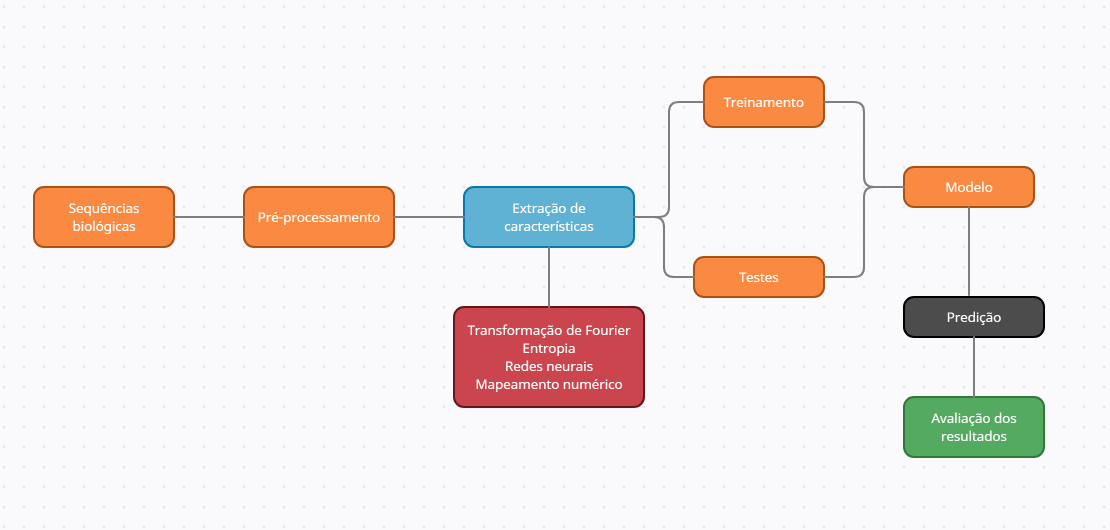
\includegraphics[width=1\textwidth]{images/fluxograma.png}
    \caption{Fluxograma de atividades criado pelo autor}
    \label{fig:workflow}
\end{figure}